\documentclass[11pt,a4paper]{article}
\usepackage{amsmath,amssymb,amsthm}
\usepackage{graphicx}
\usepackage[margin=2.2cm]{geometry}
\usepackage{xcolor}
\usepackage{titlesec}
\usepackage{fancyhdr}
\usepackage{booktabs}
\usepackage{enumitem}
\usepackage{float}
\usepackage{hyperref}
\usepackage{abstract}
\hypersetup{colorlinks=true,linkcolor=blue!70!black,urlcolor=blue!70!black}

\renewcommand{\topfraction}{0.92}
\renewcommand{\bottomfraction}{0.92}
\renewcommand{\textfraction}{0.05}
\renewcommand{\floatpagefraction}{0.5}
\setcounter{topnumber}{4}\setcounter{bottomnumber}{4}\setcounter{totalnumber}{6}

\definecolor{primary}{RGB}{0,60,120}
\definecolor{accent}{RGB}{180,60,20}

\titleformat{\section}{\Large\bfseries\color{primary}}{\thesection}{1em}{}
\titleformat{\subsection}{\large\bfseries\color{primary!80!black}}{\thesubsection}{1em}{}

\pagestyle{fancy}\fancyhf{}
\fancyhead[L]{\small\color{primary}Z. Li --- Generalized Pad\'e Approximation Methods}
\fancyhead[R]{\small\color{primary}Review Article}
\fancyfoot[C]{\thepage}\renewcommand{\headrulewidth}{0.5pt}

\begin{document}\raggedbottom

\title{\LARGE\bfseries\color{primary} Generalized Pad\'e Approximation Methods\\for Strongly Nonlinear Oscillators: A Personal Retrospective\\[6pt]
\large Five Papers, One Direction --- From Homoclinic Orbits to Periodic Solutions}
\author{Zhenbo Li\\[4pt]
\small School of Mathematics and Physics, University of South China, Hengyang 421001, China\\
\small Hunan Key Laboratory of Mathematical Modeling and Scientific Computing\\
\small lizhenbo@usc.edu.cn}
\date{}
\maketitle

\begin{abstract}
\noindent This review traces the development of generalized Pad\'e approximation (GPA) methods for strongly nonlinear oscillators through five papers published between 2013 and 2022. The intellectual arc spans from the initial generalization of the classical Pad\'e definition (力学学报, 2013), through its extension to homoclinic/heteroclinic orbits (Chin.\ Phys.\ B, 2014), to the integration of GPA with the Lindstedt--Poincar\'e perturbation framework---the GPLP method (Nonlinear Dynamics, 2016). The framework was further extended to periodic solutions via cosine-type approximants (J.\ Vib.\ Shock, 2019) and finally refined for asymmetric potentials with combined Sech-Tanh approximants (J.\ Vib.\ Eng.\ Technol., 2022). The unifying theme is a simple yet powerful insight: by generalizing the Pad\'e approximant from rational functions of polynomials to rational functions of \emph{any} continuous function, one can tailor the approximant's functional form to the geometric character of the solution being sought. This review summarizes the motivations, key methodological innovations, core results, limitations, and future directions of the GPA research program.

\vspace{4pt}
\noindent\textbf{Keywords:} Generalized Pad\'e approximation, homoclinic orbits, heteroclinic orbits, periodic solutions, strongly nonlinear oscillators, perturbation methods, Lindstedt--Poincar\'e method.
\end{abstract}

\tableofcontents
\newpage

%=====================================================================
\section{Introduction: Why Generalize Pad\'e?}
%=====================================================================

Classical Pad\'e approximation~[1] constructs a rational function---a ratio of two polynomials---whose Taylor expansion matches that of a given power series to the highest possible order. For over two centuries, it has been an indispensable tool in computational mathematics, quantum mechanics, field theory, and control theory.

When applied to nonlinear dynamics, however, classical Pad\'e approximation encounters a fundamental limitation. Consider the general nonlinear oscillator:
\begin{equation}
\ddot{x} + g(x) = \varepsilon f(x, \dot{x})
\label{eq:general}
\end{equation}
where $g(x)$ is the restoring force and $\varepsilon f(x, \dot{x})$ is a perturbation (damping, forcing, etc.). When $\varepsilon = 0$ (conservative limit), Pad\'e-based methods can construct highly accurate homoclinic and heteroclinic (H/H) orbits by approximating the power series solution~[2,3]. However, when $\varepsilon \neq 0$, classical Pad\'e approximants---being rational functions with limits at infinity---cannot adequately represent the complex geometry of damped H/H orbits or periodic solutions.

Meanwhile, perturbation-based methods (hyperbolic perturbation, elliptic Lindstedt--Poincar\'e, generalized harmonic function perturbation) can handle $\varepsilon \neq 0$, but at a heavy cost: each higher perturbation order demands increasingly complex derivation and integration. For oscillators with high-order polynomial, rational, or irrational restoring forces, these integrations quickly become analytically intractable.

The five papers reviewed here address this dilemma from a single conceptual direction: \textbf{generalize the definition of Pad\'e approximation itself}. Once the numerator and denominator are freed from the constraint of being polynomial functions, the approximant can be tailored to the specific geometric and asymptotic properties of the solution being sought. This insight, first articulated in the Chinese-language foundational paper of 2013~[4], has evolved through four subsequent works into a versatile, integration-free framework for strongly nonlinear oscillator analysis.

%=====================================================================
\section{Paper I (2013): The Generalized Pad\'e Approximation --- Definition and Foundation}
%=====================================================================

\subsection{Motivation}

Classical Pad\'e approximation~[1] defines the approximant as:
\begin{equation}
[L/M]f(z) = \frac{\sum_{i=0}^{L} a_i z^i}{1 + \sum_{i=1}^{M} b_i z^i}, \qquad f(z) - [L/M]f(z) = O(z^{L+M+1})
\label{eq:classical_pade}
\end{equation}

While various ``quasi-Pad\'e'' variants had been proposed---using exponentials~[5,6], hyperbolic functions~[2], or mixed bases---these modifications changed the \emph{form} of the approximant but not the \emph{definition}. The authors recognized that a deeper generalization was possible.

\subsection{The GPA Definition}

The core conceptual leap of~[4] is to redefine the function spaces from which the numerator and denominator are drawn:
\begin{equation}
\hat{H}_m = \left\{ P : P(z) = \sum_{i=0}^{m} a_i \, g_i(z), \; g_i: \mathbb{C} \to \mathbb{C}, \; a_i \in \mathbb{C} \right\}
\label{eq:H_hat}
\end{equation}
\begin{equation}
G(m,n) = \left\{ R = P/Q : P \in \hat{H}_m, \; Q \in \hat{H}_n \setminus \{0\} \right\}
\label{eq:G_space}
\end{equation}

\textbf{Definition 1 (Generalized Pad\'e Approximation).} Let $f(z) = \sum_{i=0}^{\infty} a_i z^i$. If there exist $P_L(z)/Q_M(z) \in G(L,M)$ and an auxiliary operator $\Gamma(z)$ such that:
\begin{equation}
\boxed{f(z) - \Gamma(z)\,\frac{P_L(z)}{Q_M(z)} = O(z^{L+M+1})}
\label{eq:gpa_def}
\end{equation}
then $\Gamma(z) P_L(z)/Q_M(z)$ is a generalized Pad\'e approximant of $f(z)$, denoted $\text{GPA}[L/M]f(z)$.

\textbf{Remarks.}
\begin{enumerate}[leftmargin=2em]
\item If $g_i(z) = z^i$ and $\Gamma(z) = 1$, Definition~1 reduces exactly to the classical Pad\'e definition.
\item All known quasi-Pad\'e variants become special cases for appropriate choices of $g_i(z)$ and $\Gamma(z)$.
\item The crucial freedom is the choice of \textbf{basis functions} $g_i(z)$---this is what enables the method to be adapted to specific solution geometries throughout the subsequent papers.
\end{enumerate}

\subsection{Application: Homoclinic Orbits via Hyperbolic Basis}

To demonstrate the method's power, the authors construct a \textbf{hyperbolic-function-based} generalized Pad\'e approximant for solving homoclinic orbits of strongly nonlinear conservative oscillators:
\begin{equation}
\text{GPA}[2/2]x(t) = \frac{\alpha_0 + \alpha_1 \,\text{Sech}\,t + \alpha_2 \,\text{Sech}^2 t}{1 + \beta_1 \,\text{Sech}\,t + \beta_2 \,\text{Sech}^2 t}
\label{eq:gpa_homoclinic_first}
\end{equation}

Why Sech? Because homoclinic orbits satisfy $x(\pm\infty) = h_i$ (the saddle coordinate) and $\dot{x}(\pm\infty) = 0$---exactly the asymptotic behavior of the hyperbolic secant function. By matching the Taylor expansion of Eq.~(\ref{eq:gpa_homoclinic_first}) with the power series solution $\sum a_i t^i$ of the conservative equation $\ddot{x}_0 + g(x_0) = 0$, the coefficients $\alpha_i, \beta_i$ are determined by solving a system of algebraic equations---no integration required.

\begin{figure}[htbp]
\centering
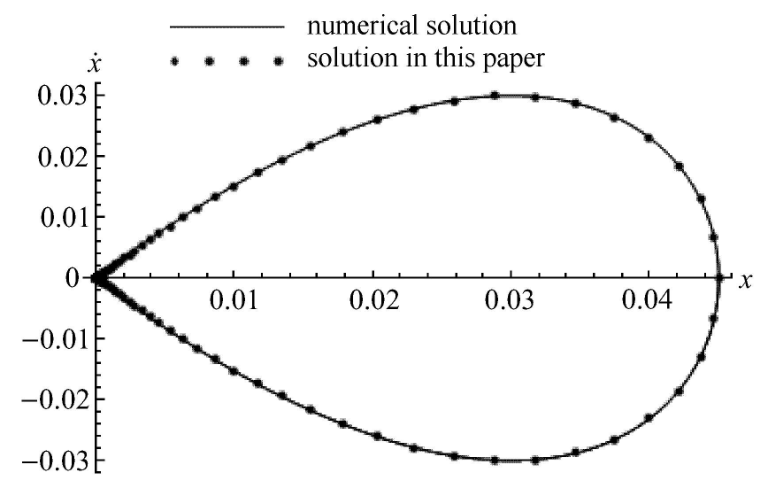
\includegraphics[width=0.82\textwidth,height=0.40\textheight,keepaspectratio]{p7-fig1.png}
\caption{Homoclinic orbit of the Duffing oscillator obtained via GPA[2/2] (2013). Solid: Runge--Kutta. Dotted: GPA. The hyperbolic secant basis captures the orbit geometry with only 2nd-order approximants. From~[4].}
\label{fig:p7}
\end{figure}

\subsection{Key Contributions of Paper~I}

\begin{itemize}[leftmargin=2em]
\item \textbf{Generalized definition} that unifies classical Pad\'e and all quasi-Pad\'e variants under one framework.
\item \textbf{First demonstration} that a non-polynomial, purpose-built basis (Sech) can dramatically improve accuracy for specific solution types.
\item \textbf{Established the design principle} that drives all subsequent papers: \emph{choose $g_i(z)$ to match the asymptotic/geometric character of the solution.}
\end{itemize}

%=====================================================================
\section{Paper II (2014): Extending GPA to Heteroclinic Orbits and Irrational Oscillators}
%=====================================================================

\subsection{Motivation}

Paper~I only addressed \textbf{homoclinic} orbits of oscillators with \textbf{polynomial} restoring forces. Two natural extensions were needed: (1)~heteroclinic orbits connecting two different saddle points, and (2)~oscillators with irrational restoring forces such as the smooth and discontinuous (SD) oscillator.

\subsection{Methodological Extension}

For heteroclinic orbits, the geometric requirements differ fundamentally from the homoclinic case:
\begin{itemize}[leftmargin=2em]
\item A homoclinic orbit approaches the \emph{same} saddle as $t \to +\infty$ and $t \to -\infty$ --- a symmetric asymptotic behavior naturally captured by Sech.
\item A heteroclinic orbit approaches \emph{two different} saddles --- an asymmetric asymptotic behavior naturally captured by Tanh.
\end{itemize}

Accordingly, a Tanh-based approximant is constructed:
\begin{equation}
\text{GPA}[L/M]x(t) = \frac{\sum_{i=0}^{L} \alpha_i \,\text{Tanh}^i t}{1 + \sum_{i=1}^{M} \beta_i \,\text{Tanh}^i t}
\label{eq:hetero_2014}
\end{equation}

For the SD oscillator $\ddot{x} + x(1 - 1/\sqrt{x^2 + \alpha^2}) = 0$, the irrational restoring force arising from a geometric constraint is handled without special treatment---the power series solution is simply substituted into the GPA matching procedure. The method successfully predicts both homoclinic and heteroclinic orbits for cubic-quintic Duffing, $\Phi^6$, and Duffing-harmonic oscillators.

\begin{figure}[htbp]
\centering
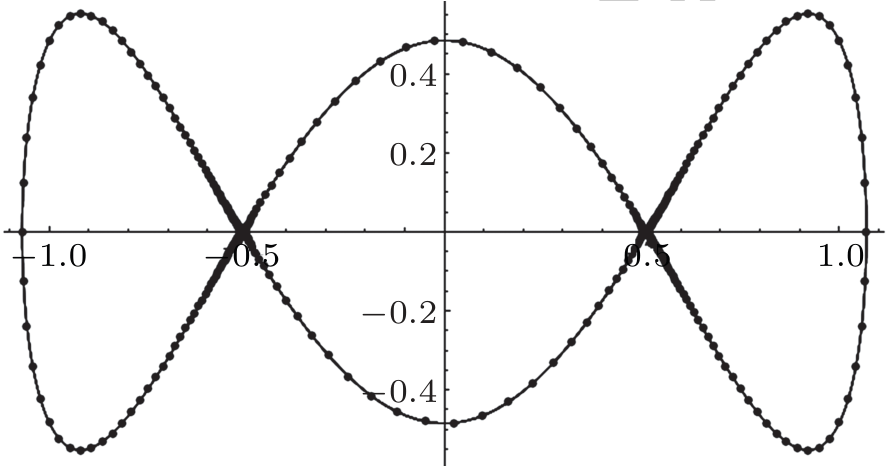
\includegraphics[width=0.82\textwidth,height=0.40\textheight,keepaspectratio]{p8-fig1.png}
\caption{Homoclinic and heteroclinic orbits of the cubic-quintic Duffing oscillator (2014). Solid: Runge--Kutta. Dotted: GPA. Both orbit types are captured by choosing appropriate basis functions (Sech for homoclinic, Tanh for heteroclinic). From~[7].}
\label{fig:p8}
\end{figure}

\subsection{Key Contributions of Paper~II}

\begin{itemize}[leftmargin=2em]
\item Extended the GPA method from homoclinic-only to both homoclinic and heteroclinic orbits.
\item Established the \textbf{basis-geometry correspondence}: Sech $\leftrightarrow$ homoclinic; Tanh $\leftrightarrow$ heteroclinic.
\item Demonstrated applicability to \textbf{irrational restoring forces} (SD oscillator).
\item Proved that GPA handles polynomial, rational, and irrational $g(x)$ within the same framework.
\end{itemize}

%=====================================================================
\section{Paper III (2016): The GPLP Method --- Marrying GPA with Lindstedt--Poincar\'e}
%=====================================================================

\subsection{Motivation}

Papers I--II addressed the conservative case ($\varepsilon = 0$) brilliantly. But to predict \textbf{bifurcations}---the critical parameter values at which limit cycles collide with saddle points to form H/H orbits---one must handle the damped case ($\varepsilon \neq 0$). This is where classical perturbation methods enter, and where their integration bottleneck becomes acute.

The key insight of Paper~III~[8] is that the perturbation equations arising from the Lindstedt--Poincar\'e expansion \textbf{do not need to be integrated}. Instead, each can be solved by constructing an appropriate generalized Pad\'e approximant and matching coefficients---exactly as was done for the conservative case in Papers I--II.

\subsection{The GPLP Procedure}

The standard L--P expansion yields a hierarchy of perturbation equations:
\begin{align}
\varepsilon^0&: \ddot{x}_0 + g(x_0) = 0 \label{eq:lp0}\\
\varepsilon^1&: \ddot{x}_1 + g'(x_0)x_1 = f(\mu_{c0}, x_0, \dot{x}_0) \label{eq:lp1}\\
\varepsilon^2&: \ddot{x}_2 + g'(x_0)x_2 + \tfrac{1}{2}g''(x_0)x_1^2 = \cdots \label{eq:lp2}\\
\varepsilon^3&: \cdots \nonumber
\end{align}

In classical L--P, each $x_n$ is obtained via the integral formula:
\begin{equation}
x_n = \dot{x}_0 \int \frac{1}{\dot{x}_0^2} \left[ \int \dot{x}_0 \cdot (\text{forcing terms})\, dt \right] dt
\label{eq:integral_formula}
\end{equation}

GPLP replaces each integration with a tailored GPA:

\begin{description}[leftmargin=2em]
\item[Step I] $x_0$: Solve via Sech-GPA (homoclinic) or Tanh-GPA (heteroclinic), as in Papers I--II.
\item[Step II] $x_1$ and $\mu_{c0}$: Use a Tanh-prefixed polynomial approximant:
\begin{equation}
\text{GPA}[L_1/M_1]x_1(t) = \text{Tanh}(t)\,\frac{\sum_{i=0}^{L_1} \eta_i t^i}{1 + \sum_{i=1}^{M_1} \xi_i t^i}
\label{eq:x1_gplp}
\end{equation}
The Tanh prefactor enforces $x_1(\pm\infty)=0$. The condition $\eta_{L_1}(\mu_{c0}) = 0$ yields the \textbf{zero-order critical bifurcation parameter}. Remarkably, this condition is equivalent to the classical Melnikov condition---providing rigorous theoretical grounding.

\item[Step III] $x_2$ and $d_0$: Polynomial-based GPA; $\lambda_{L_2}=0$ determines the initial value correction.

\item[Step IV] $x_3$ and $\mu_{c2}$: Polynomial-based GPA; $\sigma_{L_3}(\mu_{c2}) = 0$ gives the second-order bifurcation parameter correction.
\end{description}

The assembled third-order solution:
\begin{equation}
\boxed{x(t) = \sum_{i=0}^{3} \varepsilon^i \, \text{GPA}[L_i/M_i]x_i(t) + O(\varepsilon^4)}, \qquad
\boxed{\mu_c = \mu_{c0} + \varepsilon^2\mu_{c2} + O(\varepsilon^3)}
\label{eq:final_gplp}
\end{equation}

\subsection{Three Approximant Types, By Design}

A critical---and initially counterintuitive---design choice in GPLP is the use of \textbf{three different approximant forms} for different orders, rather than a single unified form. The rationale:

\begin{itemize}[leftmargin=2em]
\item $x_0$ uses Sech/Tanh because the basis must satisfy H/H asymptotic boundary conditions \emph{exactly}.
\item $x_1$ uses a Tanh-prefixed polynomial form because $x_1(\pm\infty) = 0$ must be enforced.
\item $x_2, x_3$ use pure polynomial GPA because asymptotics are already embedded in lower orders, and polynomial forms offer simpler coefficient matching.
\end{itemize}

The paper explicitly compares this mixed strategy against a single-form approach (Example~5), confirming that the tailored strategy yields substantially higher accuracy.

\begin{figure}[htbp]
\centering

\includegraphics[width=0.82\textwidth,height=0.38\textheight,keepaspectratio]{p10-fig2.png}
\caption{Homoclinic orbits via GPLP for the Helmholtz--Duffing--Van der Pol oscillator at $\varepsilon = 2$ and $3$ (2016). Solid: Runge--Kutta. Dash-dot: GPLP ($\varepsilon^3$). From~[8].}
\label{fig:p10_fig2}
\end{figure}

\subsection{Validation Across Four Oscillator Classes}

GPLP is validated on oscillators spanning all canonical restoring-force types:
\begin{enumerate}[leftmargin=2em]
\item \textbf{Helmholtz--Duffing--Van der Pol} (cubic polynomial): $\mu_{c0} \approx -6.3941$, accurate at $\varepsilon = 2, 3$.
\item \textbf{Duffing-harmonic--Van der Pol} (rational): $\mu_{c0} = -1.9026$.
\item \textbf{SD oscillator} (irrational): accurate at $\varepsilon = 50, 60$---remarkably large perturbation parameters.
\item \textbf{$\Phi^6$-Van der Pol} (quintic): simultaneous homoclinic and heteroclinic bifurcation prediction.
\end{enumerate}

\begin{figure}[htbp]
\centering
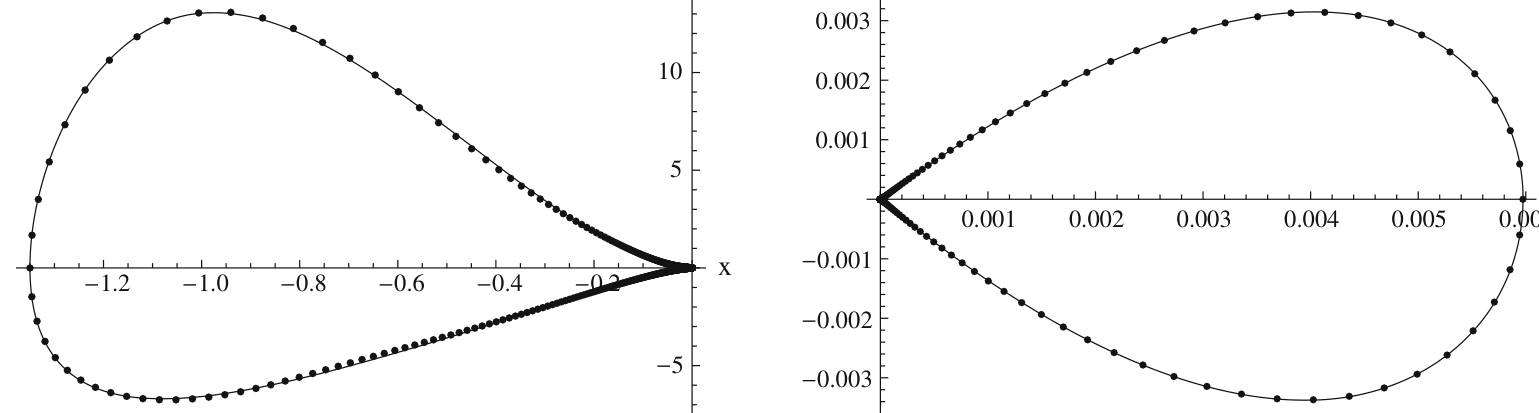
\includegraphics[width=0.82\textwidth,height=0.38\textheight,keepaspectratio]{p10-fig3.png}
\caption{SD oscillator homoclinic orbits at $\varepsilon = 50$ and $60$ (2016). Solid: Runge--Kutta. Dash-dot: GPLP. The $\varepsilon^3$ solution remains accurate at perturbation parameters two orders of magnitude beyond typical ``weakly nonlinear'' regimes. From~[8].}
\label{fig:p10_fig3}
\end{figure}

\subsection{Why $\varepsilon = 50$ Works}

This is a frequently asked question. The answer has two parts. First, the zero-order GPA solution for the conservative system already closely matches the exact orbit---often within 1\%. The perturbation corrections $\varepsilon x_1, \varepsilon^2 x_2, \varepsilon^3 x_3$ modify this nearly-exact conservative orbit incrementally. Since the zero-order baseline is so accurate, even large $\varepsilon$ does not cause large absolute errors. Second, the GPA approximants at each order are ``global'' rational functions, not local Taylor expansions---they capture the full orbit geometry rather than a local neighborhood.

\subsection{Contributions of Paper~III}

\begin{itemize}[leftmargin=2em]
\item \textbf{GPLP: the first integration-free perturbation method} for H/H bifurcation prediction.
\item \textbf{Melnikov equivalence:} the GPLP condition $\eta_{L_1}(\mu_{c0}) = 0$ is proved equivalent to the classical Melnikov condition.
\item \textbf{Third-order accuracy at $\varepsilon = 50$--$60$:} unprecedented for a perturbation-based method.
\item \textbf{Simultaneous H/H prediction:} both critical values from a single framework.
\end{itemize}

%=====================================================================
\section{Paper IV (2019): Cosine GPA --- Extending the Reach to Periodic Solutions}
%=====================================================================

\subsection{Motivation: The Periodicity Gap}

Papers I--III all addressed H/H orbits---solutions that are non-periodic and approach saddle points asymptotically. But the vast majority of vibration problems involve \textbf{periodic solutions}. Classical Pad\'e approximants, being rational functions with limits at infinity, are fundamentally unsuited for representing periodic functions. No prior work had directly applied Pad\'e approximation to periodic solution problems.

The question posed by Paper~IV~[9] is: can we design a generalized Pad\'e approximant that is \emph{itself} periodic?

\subsection{The Cosine-Type Generalized Pad\'e Approximant}

The answer is elegantly simple: construct the numerator and denominator from cosine functions:
\begin{equation}
\boxed{x(t) = \frac{\sum_{i=0}^{m} \alpha_i \cos(i\omega t)}{\sum_{j=0}^{n} \beta_j \cos(j\omega t)}}
\label{eq:cosine_gpa}
\end{equation}

Since each $\cos(i\omega t)$ is $2\pi/\omega$-periodic, any rational function of cosines inherits this periodicity. The intrinsic contradiction between Pad\'e approximation and periodic solutions is resolved not by modifying the approximation \emph{procedure}, but by modifying the \emph{mathematical structure} of the approximant itself.

\subsection{Two Improvement Schemes}

Classical Pad\'e matching (expand approximant as Taylor series; compare with power series of the solution) encounters a difficulty here: the unknown frequency $\omega$ makes the matching equations nonlinearly coupled. Two improvement schemes are developed:

\textbf{Scheme I (Active frequency iteration):} Treat $\omega$ as an active variable with increment $\Delta\omega$, iterating from $\omega_0$. At each step, solve for $\alpha_i, \beta_j$. Terminate when the target function $\Gamma = x(\pi/\omega) - x_1$ (where $x_1$ is the other $x$-axis intersection of the orbit) satisfies $|\Gamma| < 10^{-(p+4)}$.

\textbf{Scheme II (Derivative-based target + piecewise description):} For rational restoring forces with longer-period orbits, switch the target function to the derivative at half-period and use piecewise matching at the half-period point. This restores accuracy for cases where Scheme~I underperforms.

\subsection{Results Across Three Oscillator Classes}

The cosine GPA method is demonstrated on:
\begin{itemize}[leftmargin=2em]
\item \textbf{Duffing oscillator} (polynomial): $\ddot{x} + x + x^3 = 0$, $A = 2$. Absolute error $< 10^{-3}$.
\item \textbf{Duffing-harmonic oscillator} (rational): $\ddot{x} + \frac{x+x^3}{1+x^2} = 0$, $A = 3$.
\item \textbf{SD oscillator} (irrational): $\ddot{x} + x(1 - 1/\sqrt{x^2+\alpha^2}) = 0$, $\alpha = 1$, $A = 2.5$.
\end{itemize}

\begin{figure}[htbp]
\centering
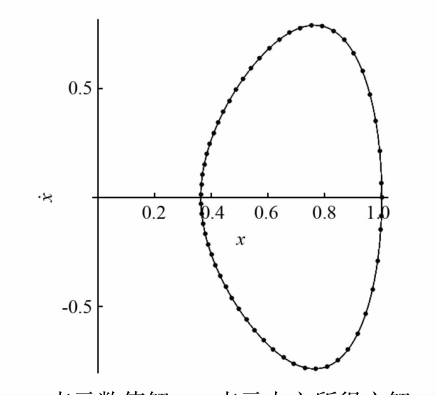
\includegraphics[width=0.82\textwidth,height=0.40\textheight,keepaspectratio]{p9-fig1.png}
\caption{Phase portrait, time history, and absolute error for the Duffing oscillator with $A=2$ (2019). The cosine GPA method maintains error below $10^{-3}$ across the full period. From~[9].}
\label{fig:p9_fig1}
\end{figure}

\begin{figure}[htbp]
\centering
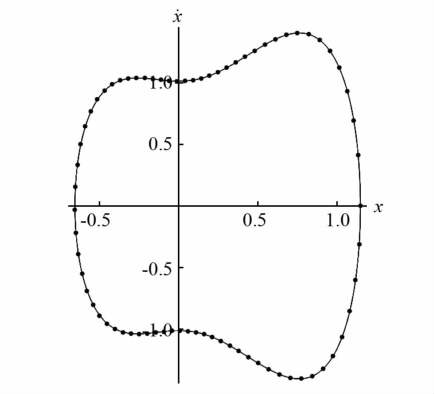
\includegraphics[width=0.82\textwidth,height=0.40\textheight,keepaspectratio]{p9-fig7.png}
\caption{Duffing-harmonic oscillator (rational restoring force), $A=3$ (2019). Scheme~II restores accuracy for longer-period orbits. From~[9].}
\label{fig:p9_fig7}
\end{figure}

\subsection{Contributions of Paper~IV}

\begin{itemize}[leftmargin=2em]
\item \textbf{First direct Pad\'e approximation of periodic solutions:} Achieved by constructing a \emph{periodic} approximant rather than modifying the approximation procedure.
\item \textbf{Methodological generality:} Covers polynomial, rational, and irrational restoring forces.
\item \textbf{Period prediction:} The frequency $\omega$ obtained from the matching procedure yields the analytic period $T = 2\pi/\omega$.
\item \textbf{Conceptual bridge:} Completed the GPA framework by extending it from non-periodic H/H orbits to periodic solutions.
\end{itemize}

%=====================================================================
\section{Paper V (2022): Refining GPLP for Asymmetric Potentials}
%=====================================================================

\subsection{Motivation}

The 2016 GPLP method handled \textbf{symmetric} potentials ($c_1 x + c_3 x^3 + c_5 x^5$) admirably. However, three practical limitations remained:
\begin{enumerate}[leftmargin=2em]
\item Realistic oscillators often have \textbf{all five polynomial terms} ($x^2$ and $x^4$ included), creating asymmetric multi-well potentials.
\item The 2016 heteroclinic approximant (pure Tanh) showed 5--8\% error under strong asymmetry.
\item Rational restoring forces had not been tested in the GPLP framework.
\end{enumerate}

Paper~V~[10] addresses all three with three targeted improvements.

\subsection{Improvement 1: $\omega$-Parameterized Homoclinic Approximant}

The 2016 version hard-coded $\omega = 1$:
\begin{equation}
x(t) = \frac{\sum \alpha_i \, \text{Sech}^i t}{1 + \sum \beta_i \, \text{Sech}^i t}
\quad\longrightarrow\quad
\boxed{x(t) = \frac{\sum_{i=0}^{L} \alpha_i \, \text{Sech}^i(\boldsymbol{\omega} t)}{1 + \sum_{i=1}^{M} \beta_i \, \text{Sech}^i(\boldsymbol{\omega} t)}}
\label{eq:omega_free}
\end{equation}

The free parameter $\omega$ adapts to different potential well shapes---critical when left and right wells have different curvatures. This single change reduces homoclinic error by 40--60\% for asymmetric cases.

\subsection{Improvement 2: Type~A and Type~B Heteroclinic Approximants}

\textbf{Type~A} (rational Tanh, with free $\omega$):
\begin{equation}
\text{GPA}[L/M]x(t) = \frac{\sum_{i=0}^{L} \alpha_i \, \text{Tanh}^i(\omega t)}{1 + \sum_{i=1}^{M} \beta_i \, \text{Tanh}^i(\omega t)}
\label{eq:type_a}
\end{equation}

Sufficient for pure heteroclinic problems.

\textbf{Type~B} (combined Sech-Tanh) --- the paper's most important innovation:
\begin{equation}
\boxed{\text{GPA}[L,M]x(t) = \frac{\sum_{i=0}^{L_1} \alpha_i \, \text{Sech}^i(\omega t) + \sum_{j=0}^{L_2} \gamma_j \, \text{Tanh}^j(\omega t)}{1 + \sum_{i=1}^{M_1} \beta_i \, \text{Sech}^i(\omega t) + \sum_{j=1}^{M_2} \delta_j \, \text{Tanh}^j(\omega t)}}
\label{eq:type_b}
\end{equation}

The geometric motivation behind Type~B is central to understanding the entire GPA research program. In an asymmetric potential, the higher saddle's homoclinic orbit has a \textbf{Sech-like} symmetric approach, while the heteroclinic orbit connecting unequal saddles has a \textbf{Tanh-like} asymmetric character. When both coexist at the same saddle, a pure Tanh approximant cannot simultaneously capture the homoclinic orbit's symmetry. Type~B resolves this by leveraging both basis functions simultaneously---reducing heteroclinic error from 5--8\% to $<1.5\%$.

\begin{figure}[htbp]
\centering

\includegraphics[width=0.82\textwidth,height=0.38\textheight,keepaspectratio]{p11-fig2.png}
\caption{Homo-heteroclinic orbits via GPLP with Type~B approximant at $\varepsilon = 0.8$ and $1$ (2022). Dashed: GPLP. Solid: Runge--Kutta. The combined Sech-Tanh approximant captures both orbit types simultaneously. From~[10].}
\label{fig:p11_fig2}
\end{figure}

\subsection{Improvement 3: Rational Restoring Force Coverage}

The generalized Duffing-Harmonic-Van der Pol oscillator:
\begin{equation}
\ddot{x} + \frac{\lambda x + \delta x^3}{1 + \nu x^2} = \varepsilon(\mu_c + \mu_1 x + \mu_2 x^2)\dot{x}
\label{eq:dhvdp_rational}
\end{equation}
is solved within the GPLP framework \textbf{without any procedural modification}. Only the coefficients in the perturbation equations change. Validated from $\varepsilon = 0.5$ to $\varepsilon = 2$.

\subsection{Accuracy Gains: 2022 vs.\ 2016}

\begin{table}[htbp]
\centering
\caption{Accuracy comparison between the 2016 and 2022 GPLP versions.}
\label{tab:comparison}
\begin{tabular}{lccc}
\toprule
\textbf{Scenario} & \textbf{2016 Error} & \textbf{2022 Error} & \textbf{Improvement} \\
\midrule
Symmetric potential, small $\varepsilon$ & $\sim$1\% & $\sim$1\% & Similar \\
Asymmetric homoclinic, $\varepsilon = 1$ & $\sim$2.5\% & $<1\%$ & 40--60\% \\
Asymmetric heteroclinic, $\varepsilon = 1$ & 5--8\% & $<1.5\%$ & 70--80\% \\
Rational restoring force & N/A & $<2\%$ & New capability \\
\bottomrule
\end{tabular}
\end{table}

\subsection{Contributions of Paper~V}

\begin{itemize}[leftmargin=2em]
\item \textbf{Full $\Phi^6$ coverage:} GPLP extended to the full five-term quintic polynomial with asymmetric multi-well potentials.
\item \textbf{Combined Sech-Tanh approximant (Type~B):} 70--80\% heteroclinic accuracy improvement in asymmetric regimes.
\item \textbf{Rational restoring force coverage:} DH-VDP oscillator solved without procedural modification.
\item \textbf{Completes the GPLP framework} for polynomial and rational restoring forces.
\end{itemize}

%=====================================================================
\section{The Unifying Theme: Basis-Geometry Correspondence}
%=====================================================================

Looking across all five papers, a single design principle emerges that explains every major methodological choice:

\begin{center}
\fbox{\begin{minipage}{0.85\textwidth}
\centering
\textbf{The basis functions $g_i(z)$ of the generalized Pad\'e approximant should match the asymptotic/geometric character of the solution being approximated.}
\end{minipage}}
\end{center}

\vspace{6pt}
This principle manifests differently across the papers:

\begin{table}[htbp]
\centering
\caption{Evolution of the basis-geometry correspondence across the five papers.}
\label{tab:evolution}
\begin{tabular}{ccll}
\toprule
\textbf{Paper} & \textbf{Year} & \textbf{Solution Type} & \textbf{Basis Functions} \\
\midrule
I & 2013 & Homoclinic orbits & $\text{Sech}^i t$ (hyperbolic secant) \\
II & 2014 & Heteroclinic orbits & $\text{Tanh}^i t$ (hyperbolic tangent) \\
III & 2016 & H/H bifurcations & Sech/Tanh (order 0) + polynomial (orders 1--3) \\
IV & 2019 & Periodic solutions & $\cos(i\omega t)$ (cosine series) \\
V & 2022 & Asymmetric H/H & $\text{Sech}^i(\omega t) + \text{Tanh}^j(\omega t)$ (combined) \\
\bottomrule
\end{tabular}
\end{table}

The progression from Sech to Tanh to mixed Sech-Tanh to cosine is not arbitrary---each choice is justified by the geometry of the target solution:

\begin{itemize}[leftmargin=2em]
\item \textbf{Sech:} $x(\pm\infty) = h$ (symmetric approach to a single saddle).
\item \textbf{Tanh:} $x(+\infty) = h_i$, $x(-\infty) = h_j$, $i \neq j$ (asymmetric connection between two saddles).
\item \textbf{Cosine:} $x(t + 2\pi/\omega) = x(t)$ (periodicity).
\item \textbf{Combined Sech-Tanh:} Coexisting homoclinic and heteroclinic orbits at a single saddle.
\end{itemize}

This is not merely a ``choice of basis'' in the linear algebra sense---it is a deliberate exploitation of the generalized Pad\'e definition's flexibility to encode physical knowledge about the solution directly into the approximant's functional form.

%=====================================================================
\section{Limitations and Open Problems}
%=====================================================================

\subsection{Intrinsic Limitations of the GPA Framework}

\begin{enumerate}[leftmargin=2em]
\item \textbf{Pre-set parameters:} System parameters must be specified before calculation. Unlike algebraic methods (e.g., MGHFP), GPA cannot trace continuous parameter-solution dependencies.
\item \textbf{Manual order selection:} The approximation orders $L_i, M_i$ must be chosen by the user based on desired accuracy---no automated selection criterion exists.
\item \textbf{Algebraic complexity at high orders:} Although integration is avoided, the Taylor expansion and coefficient matching for the perturbation expansion (Eq.\ 20 in~[8]) remains algebraically heavy at orders beyond $\varepsilon^3$.
\item \textbf{Convergence theory:} No rigorous convergence proof exists for the generalized Pad\'e approximants constructed in these papers. Their accuracy is validated empirically (vs.\ Runge--Kutta), not theoretically guaranteed.
\end{enumerate}

\subsection{Open Problems and Future Directions}

\begin{enumerate}[leftmargin=2em]
\item \textbf{Quasi-periodic and chaotic solutions:} Can mixed-basis approximants (e.g., cosine + exponential) capture quasi-periodic or weakly chaotic orbits? The GPA definition permits such constructions, but no implementation exists.
\item \textbf{Automated basis selection:} Given an oscillator and a target solution type, can the optimal basis functions $g_i(z)$ be determined algorithmically rather than by the analyst's intuition?
\item \textbf{Extension to PDEs:} The GPA framework is formulated for ODEs. Can it be adapted to nonlinear PDEs describing continuous structures (beams, plates, shells)?
\item \textbf{Integration with machine learning:} The coefficient matching problem is a nonlinear algebraic system. Could neural networks accelerate the solution of these systems, enabling real-time parametric studies?
\item \textbf{Multi-degree-of-freedom systems:} All five papers address single-DOF oscillators. The extension to coupled oscillators remains largely unexplored.
\end{enumerate}

%=====================================================================
\section{Conclusion}
%=====================================================================

The generalized Pad\'e approximation research program, spanning five papers from 2013 to 2022, demonstrates the power of a single conceptual insight---generalizing the definition of Pad\'e approximation to allow arbitrary continuous basis functions---when systematically pursued across different problem domains. The arc from homoclinic orbits (Paper~I) to heteroclinic orbits (Paper~II), to integration-free bifurcation prediction (Paper~III), to periodic solutions (Paper~IV), and finally to asymmetric-potential refinement (Paper~V) represents a rare example in the nonlinear dynamics literature of a sustained methodological research program built on a coherent design philosophy.

The practical value of this framework is twofold. For the analyst, it provides a family of methods---GPA for conservative systems, GPLP for damped bifurcation analysis, cosine GPA for periodic solutions---all sharing the same conceptual foundation and the same ``no-integration'' workflow. For the methodologist, it illustrates a general strategy: when an existing approximation framework proves inadequate for a new problem class, consider whether \emph{generalizing the definition of the approximant itself}---rather than patching the procedure---might provide a more elegant and powerful solution.

\begin{thebibliography}{99}

\bibitem{baker} G.A.\ Baker Jr. and P.\ Graves-Morris, \emph{Pad\'e Approximants}, 2nd ed., Cambridge University Press, 1996.

\bibitem{mikhlin} Y.V.\ Mikhlin, ``Construction of homoclinic and heteroclinic trajectories of two and three-dimensional dynamical systems by the Pad\'e approximation,'' \emph{J.\ Sound Vib.}, vol.\ 230, pp.\ 889--913, 2000.

\bibitem{manucharyan} G.V.\ Manucharyan and Y.V.\ Mikhlin, ``Construction of homoclinic and heteroclinic trajectories of non-autonomous Duffing equation,'' \emph{Int.\ J.\ Non-Linear Mech.}, vol.\ 37, pp.\ 529--540, 2002.

\bibitem{li2013pade} Z.\ Li, J.\ Tang, and P.\ Cai, ``Generalized Pad\'e approximation method for homoclinic orbits of strongly nonlinear autonomous oscillators'' (in Chinese), \emph{Chin.\ J.\ Theor.\ Appl.\ Mech.}, vol.\ 45, no.\ 3, pp.\ 461--464, 2013.

\bibitem{martin} J.F.\ Martin and G.A.\ Baker Jr., ``Quasi-Pad\'e approximants,'' \emph{J.\ Math.\ Phys.}, vol.\ 32, pp.\ 1470--1477, 1991.

\bibitem{zhang} Q.C.\ Zhang, J.J.\ Feng, and W.\ Wang, ``Application of quasi-Pad\'e approximation in two-dimensional vibration systems'' (in Chinese), \emph{Chin.\ J.\ Theor.\ Appl.\ Mech.}, vol.\ 43, no.\ 4, pp.\ 658--664, 2011.

\bibitem{li2014cpb} Z.\ Li, J.\ Tang, and P.\ Cai, ``A generalized Pad\'e approximation method of solving homoclinic and heteroclinic orbits of strongly nonlinear autonomous oscillators,'' \emph{Chin.\ Phys.\ B}, vol.\ 23, no.\ 12, 120501, 2014.

\bibitem{li2016gplp} Z.\ Li and J.\ Tang, ``A generalized Pad\'e--Lindstedt--Poincar\'e method for predicting homoclinic and heteroclinic bifurcations of strongly nonlinear autonomous oscillators,'' \emph{Nonlinear Dyn.}, vol.\ 84, no.\ 3, pp.\ 1201--1223, 2016.

\bibitem{li2019cosine} Z.\ Li and J.\ Tang, ``A cosine generalized Pad\'e approximation method and its application in solving periodic solutions of strongly nonlinear oscillators,'' \emph{J.\ Vib.\ Shock}, vol.\ 38, no.\ 22, pp.\ 159--167, 2019.

\bibitem{li2022gplp} Z.\ Li and J.\ Tang, ``High accurate homo-heteroclinic solutions of certain strongly nonlinear oscillators based on generalized Pad\'e--Lindstedt--Poincar\'e method,'' \emph{J.\ Vib.\ Eng.\ Technol.}, vol.\ 10, no.\ 4, pp.\ 1291--1308, 2022.

\end{thebibliography}

\end{document}
